Nous entamons à présent la phase d’analyse du sprint 1.2. Cette section présente le diagramme de cas d’utilisation correspondant aux fonctionnalités ciblées durant ce sprint, accompagné de descriptions textuelles détaillées pour certains cas d’usage.

\subsubsection{Diagramme de cas d’utilisation du sprint 1.2}

La figure \ref{fig:caseS2} illustre le diagramme de cas d’utilisation raffiné du sprint 1.2. Il met en avant les différents cas d’usage planifiés pour ce sprint, en mettant l’accent sur les interactions entre les utilisateurs et les composants du système.

\begin{figure}[H]
\centering
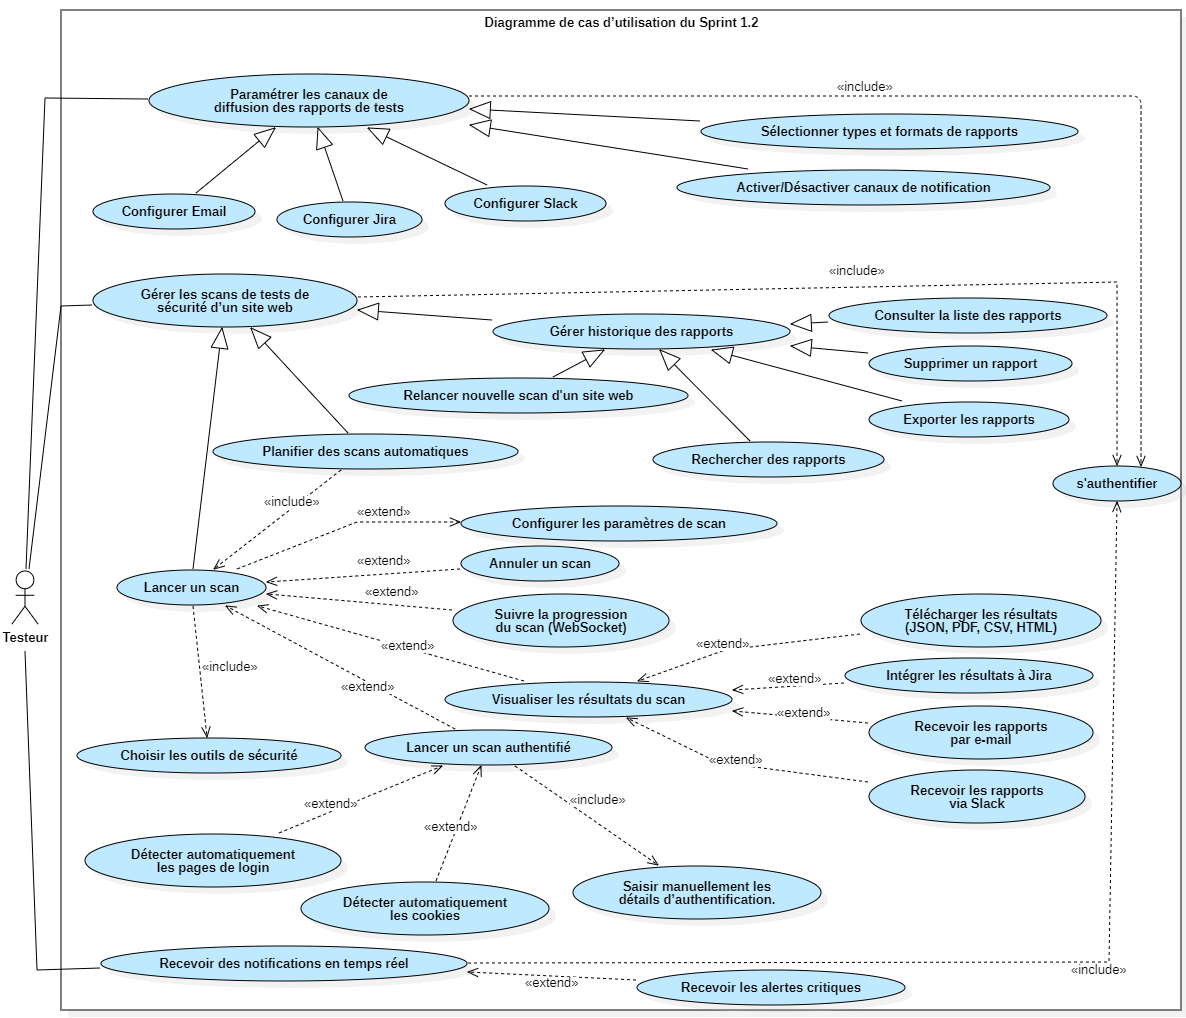
\includegraphics[width=\linewidth]{chapitres/ch3Sp1/section/sprint2/img/LastUseCaseSprint1.2.png}
\caption{Diagramme de cas d’utilisation du sprint 1.2}
\label{fig:caseS2}
\end{figure}
\vspace{-0.6cm}
\subsubsection{Raffinement des cas d’utilisation}
Cette phase d’affinement a permis de clarifier les interactions entre les acteurs et le système, d’identifier les éventuelles dépendances fonctionnelles, et de décomposer les fonctionnalités complexes en sous-cas d’utilisation plus précis.
\begin{enumerate}[label=\alph*), left=-0.1cm]
    \item \textbf{Description textuelle du cas d’utilisation "Choisir les outils de sécurité}\\
        Le tableau ~\ref{tab:tools-select}  présente la description textuelle du cas d’utilisation "Choisir les outils de sécurité".
                  \begin{spacing}{1}
                        \begin{longtable}{|p{0.12\linewidth}|p{0.88\linewidth}|}
                            \caption{Description textuelle du cas d’utilisation : Choisir les outils de sécurité}
                            \label{tab:tools-select}\\
                            \hline
                            \textbf{Titre} & Choisir les outils de sécurité \\
                            \hline
                            \textbf{Acteur} & Testeur \\
                            \hline
                            \textbf{Résumé} & Ce cas d'utilisation permet au testeur de sélectionner les outils qu’il souhaite utiliser pour les futurs scans et enregistre cette configuration pour la réutiliser. \\
                            \hline
                            \textbf{Pré-conditions} & Le testeur est connecté. Les outils disponibles sont listés dynamiquement depuis le backend. \\
                            \hline
                            \textbf{Post-conditions} & Les préférences du testeur sont enregistrées en base de données et réutilisées automatiquement dans les scans suivants. \\
                            \hline
                            \textbf{Scénario nominal} & 
                            \begin{minipage}{\linewidth}
                                \vspace{0.1cm}
                                \begin{enumerate}[label=\arabic*., left=0.1cm]
                                    \item L'utilisateur accède à l’interface de sélection.
                                    \item Il choisit les outils à utiliser via des cases à cocher. 
                                    \item Il valide sa sélection. 
                                    \item Le backend enregistre la configuration. 
                                    \item Un message de confirmation apparaît. 
                                \end{enumerate}
                                \vspace{0.1cm}
                            \end{minipage}\\
                            \hline
                            \textbf{Scénario d’erreur} &
                            \begin{minipage}{\linewidth}
                                \vspace{0.1cm}
                                \begin{itemize}[left=0cm]
                                    \item[\textbullet] \textbf{Étape 3 (Informations incomplètes):}
                                    \begin{itemize}[label=\ding{56}]
                                        \item Si aucun outil n’est sélectionné alors le système affiche un message d’erreur .
                                    \end{itemize}
                        
                                    \item[\textbullet] \textbf{Étape 4 (Erreur d'enregistrement):}
                                    \begin{itemize}[label=\ding{56}]
                                        \item En cas d’échec lors de l’enregistrement des données, le système affiche un message d’erreur "préférences non enregistrées" et invite à réessayer ultérieurement.
                                    \end{itemize}
                                \end{itemize}
                                \vspace{0.1cm}
                            \end{minipage}\\
                            \hline
                        \end{longtable}
                    \end{spacing}
                  \vspace{-0.2cm}
\end{enumerate}



